% Created by tikzDevice version 0.12.5 on 2023-11-24 23:42:35
% !TEX encoding = UTF-8 Unicode
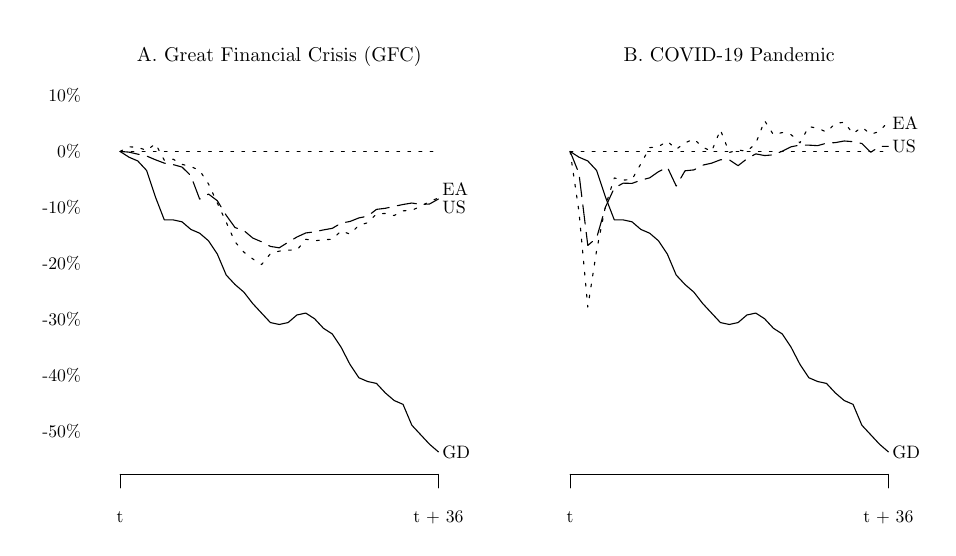
\begin{tikzpicture}[x=1pt,y=1pt]
\definecolor{fillColor}{RGB}{255,255,255}
\path[use as bounding box,fill=fillColor,fill opacity=0.00] (0,0) rectangle (325.21,180.67);
\begin{scope}
\path[clip] ( 28.80, 19.20) rectangle (153.01,161.47);
\definecolor{drawColor}{RGB}{0,0,0}

\path[draw=drawColor,line width= 0.4pt,line join=round,line cap=round] ( 33.40,135.94) --
	( 36.59,133.88) --
	( 39.79,132.50) --
	( 42.98,129.07) --
	( 46.18,119.45) --
	( 49.37,111.21) --
	( 52.57,111.21) --
	( 55.76,110.52) --
	( 58.96,107.77) --
	( 62.15,106.40) --
	( 65.35,103.65) --
	( 68.54, 98.84) --
	( 71.74, 91.28) --
	( 74.93, 87.85) --
	( 78.13, 85.10) --
	( 81.32, 80.98) --
	( 84.51, 77.54) --
	( 87.71, 74.11) --
	( 90.90, 73.42) --
	( 94.10, 74.11) --
	( 97.29, 76.85) --
	(100.49, 77.54) --
	(103.68, 75.48) --
	(106.88, 72.04) --
	(110.07, 69.99) --
	(113.27, 65.17) --
	(116.46, 58.99) --
	(119.66, 54.18) --
	(122.85, 52.81) --
	(126.04, 52.12) --
	(129.24, 48.69) --
	(132.43, 45.94) --
	(135.63, 44.56) --
	(138.82, 37.01) --
	(142.02, 33.57) --
	(145.21, 30.14) --
	(148.41, 27.39);
\end{scope}
\begin{scope}
\path[clip] ( 28.80, 19.20) rectangle (153.01,161.47);
\definecolor{drawColor}{RGB}{0,0,0}

\path[draw=drawColor,line width= 0.4pt,dash pattern=on 1pt off 3pt ,line join=round,line cap=round] ( 33.40,135.94) --
	(148.41,135.94);
\end{scope}
\begin{scope}
\path[clip] (  0.00,  0.00) rectangle (325.21,180.67);
\definecolor{drawColor}{RGB}{0,0,0}

\path[draw=drawColor,line width= 0.4pt,line join=round,line cap=round] ( 33.40, 19.20) -- (148.41, 19.20);

\path[draw=drawColor,line width= 0.4pt,line join=round,line cap=round] ( 33.40, 19.20) -- ( 33.40, 14.40);

\path[draw=drawColor,line width= 0.4pt,line join=round,line cap=round] (148.41, 19.20) -- (148.41, 14.40);

\node[text=drawColor,anchor=base,inner sep=0pt, outer sep=0pt, scale=  0.64] at ( 33.40,  1.92) {t};

\node[text=drawColor,anchor=base,inner sep=0pt, outer sep=0pt, scale=  0.64] at (148.41,  1.92) {t + 36};

\node[text=drawColor,anchor=base east,inner sep=0pt, outer sep=0pt, scale=  0.64] at ( 19.20, 32.40) {-50\%};

\node[text=drawColor,anchor=base east,inner sep=0pt, outer sep=0pt, scale=  0.64] at ( 19.20, 52.67) {-40\%};

\node[text=drawColor,anchor=base east,inner sep=0pt, outer sep=0pt, scale=  0.64] at ( 19.20, 72.93) {-30\%};

\node[text=drawColor,anchor=base east,inner sep=0pt, outer sep=0pt, scale=  0.64] at ( 19.20, 93.20) {-20\%};

\node[text=drawColor,anchor=base east,inner sep=0pt, outer sep=0pt, scale=  0.64] at ( 19.20,113.47) {-10\%};

\node[text=drawColor,anchor=base east,inner sep=0pt, outer sep=0pt, scale=  0.64] at ( 19.20,133.73) {0\%};

\node[text=drawColor,anchor=base east,inner sep=0pt, outer sep=0pt, scale=  0.64] at ( 19.20,154.00) {10\%};

\node[text=drawColor,anchor=base west,inner sep=0pt, outer sep=0pt, scale=  0.65] at (149.84, 25.15) {GD};
\end{scope}
\begin{scope}
\path[clip] ( 28.80, 19.20) rectangle (153.01,161.47);
\definecolor{drawColor}{RGB}{0,0,0}

\path[draw=drawColor,line width= 0.4pt,dash pattern=on 7pt off 3pt ,line join=round,line cap=round] ( 33.40,135.94) --
	( 36.59,135.70) --
	( 39.79,134.96) --
	( 42.98,134.30) --
	( 46.18,132.93) --
	( 49.37,131.72) --
	( 52.57,131.19) --
	( 55.76,130.31) --
	( 58.96,127.19) --
	( 62.15,118.69) --
	( 65.35,120.55) --
	( 68.54,118.12) --
	( 71.74,112.88) --
	( 74.93,108.43) --
	( 78.13,107.36) --
	( 81.32,104.66) --
	( 84.51,103.29) --
	( 87.71,101.63) --
	( 90.90,101.12) --
	( 94.10,103.13) --
	( 97.29,105.02) --
	(100.49,106.49) --
	(103.68,106.89) --
	(106.88,107.59) --
	(110.07,108.16) --
	(113.27,110.04) --
	(116.46,110.64) --
	(119.66,111.92) --
	(122.85,112.55) --
	(126.04,115.01) --
	(129.24,115.40) --
	(132.43,116.10) --
	(135.63,116.77) --
	(138.82,117.30) --
	(142.02,116.80) --
	(145.21,116.95) --
	(148.41,118.74);
\end{scope}
\begin{scope}
\path[clip] (  0.00,  0.00) rectangle (325.21,180.67);
\definecolor{drawColor}{RGB}{0,0,0}

\node[text=drawColor,anchor=base west,inner sep=0pt, outer sep=0pt, scale=  0.65] at (149.84,113.43) {US};
\end{scope}
\begin{scope}
\path[clip] ( 28.80, 19.20) rectangle (153.01,161.47);
\definecolor{drawColor}{RGB}{0,0,0}

\path[draw=drawColor,line width= 0.4pt,dash pattern=on 1pt off 3pt ,line join=round,line cap=round] ( 33.40,135.94) --
	( 36.59,137.62) --
	( 39.79,137.43) --
	( 42.98,136.31) --
	( 46.18,138.74) --
	( 49.37,132.77) --
	( 52.57,133.14) --
	( 55.76,131.27) --
	( 58.96,130.53) --
	( 62.15,129.03) --
	( 65.35,124.18) --
	( 68.54,117.28) --
	( 71.74,110.37) --
	( 74.93,103.28) --
	( 78.13, 99.55) --
	( 81.32, 97.12) --
	( 84.51, 95.07) --
	( 87.71, 98.99) --
	( 90.90, 99.92) --
	( 94.10,100.29) --
	( 97.29,100.29) --
	(100.49,104.21) --
	(103.68,103.65) --
	(106.88,104.03) --
	(110.07,104.21) --
	(113.27,107.20) --
	(116.46,106.08) --
	(119.66,109.25) --
	(122.85,110.18) --
	(126.04,113.36) --
	(129.24,113.54) --
	(132.43,112.80) --
	(135.63,114.48) --
	(138.82,114.66) --
	(142.02,116.16) --
	(145.21,117.84) --
	(148.41,119.14);
\end{scope}
\begin{scope}
\path[clip] (  0.00,  0.00) rectangle (325.21,180.67);
\definecolor{drawColor}{RGB}{0,0,0}

\node[text=drawColor,anchor=base west,inner sep=0pt, outer sep=0pt, scale=  0.65] at (149.84,119.92) {EA};
\end{scope}
\begin{scope}
\path[clip] (  0.00,  0.00) rectangle (162.61,180.67);
\definecolor{drawColor}{RGB}{0,0,0}

\node[text=drawColor,anchor=base,inner sep=0pt, outer sep=0pt, scale=  0.72] at ( 90.90,168.60) {A. Great Financial Crisis (GFC)};
\end{scope}
\begin{scope}
\path[clip] (191.41, 19.20) rectangle (315.62,161.47);
\definecolor{drawColor}{RGB}{0,0,0}

\path[draw=drawColor,line width= 0.4pt,line join=round,line cap=round] (196.01,135.94) --
	(199.20,133.88) --
	(202.40,132.50) --
	(205.59,129.07) --
	(208.79,119.45) --
	(211.98,111.21) --
	(215.18,111.21) --
	(218.37,110.52) --
	(221.56,107.77) --
	(224.76,106.40) --
	(227.95,103.65) --
	(231.15, 98.84) --
	(234.34, 91.28) --
	(237.54, 87.85) --
	(240.73, 85.10) --
	(243.93, 80.98) --
	(247.12, 77.54) --
	(250.32, 74.11) --
	(253.51, 73.42) --
	(256.71, 74.11) --
	(259.90, 76.85) --
	(263.10, 77.54) --
	(266.29, 75.48) --
	(269.48, 72.04) --
	(272.68, 69.99) --
	(275.87, 65.17) --
	(279.07, 58.99) --
	(282.26, 54.18) --
	(285.46, 52.81) --
	(288.65, 52.12) --
	(291.85, 48.69) --
	(295.04, 45.94) --
	(298.24, 44.56) --
	(301.43, 37.01) --
	(304.63, 33.57) --
	(307.82, 30.14) --
	(311.01, 27.39);
\end{scope}
\begin{scope}
\path[clip] (191.41, 19.20) rectangle (315.62,161.47);
\definecolor{drawColor}{RGB}{0,0,0}

\path[draw=drawColor,line width= 0.4pt,dash pattern=on 1pt off 3pt ,line join=round,line cap=round] (196.01,135.94) --
	(311.01,135.94);
\end{scope}
\begin{scope}
\path[clip] (  0.00,  0.00) rectangle (325.21,180.67);
\definecolor{drawColor}{RGB}{0,0,0}

\path[draw=drawColor,line width= 0.4pt,line join=round,line cap=round] (196.01, 19.20) -- (311.01, 19.20);

\path[draw=drawColor,line width= 0.4pt,line join=round,line cap=round] (196.01, 19.20) -- (196.01, 14.40);

\path[draw=drawColor,line width= 0.4pt,line join=round,line cap=round] (311.01, 19.20) -- (311.01, 14.40);

\node[text=drawColor,anchor=base,inner sep=0pt, outer sep=0pt, scale=  0.64] at (196.01,  1.92) {t};

\node[text=drawColor,anchor=base,inner sep=0pt, outer sep=0pt, scale=  0.64] at (311.01,  1.92) {t + 36};

\node[text=drawColor,anchor=base west,inner sep=0pt, outer sep=0pt, scale=  0.65] at (312.45, 25.15) {GD};
\end{scope}
\begin{scope}
\path[clip] (191.41, 19.20) rectangle (315.62,161.47);
\definecolor{drawColor}{RGB}{0,0,0}

\path[draw=drawColor,line width= 0.4pt,dash pattern=on 7pt off 3pt ,line join=round,line cap=round] (196.01,135.94) --
	(199.20,128.03) --
	(202.40,101.97) --
	(205.59,104.71) --
	(208.79,115.86) --
	(211.98,122.74) --
	(215.18,124.48) --
	(218.37,124.40) --
	(221.56,125.56) --
	(224.76,126.41) --
	(227.95,128.64) --
	(231.15,130.26) --
	(234.34,123.46) --
	(237.54,128.96) --
	(240.73,129.27) --
	(243.93,130.99) --
	(247.12,131.70) --
	(250.32,132.93) --
	(253.51,132.93) --
	(256.71,130.81) --
	(259.90,133.29) --
	(263.10,135.07) --
	(266.29,134.45) --
	(269.48,134.72) --
	(272.68,136.03) --
	(275.87,137.62) --
	(279.07,138.26) --
	(282.26,138.22) --
	(285.46,138.04) --
	(288.65,138.93) --
	(291.85,139.13) --
	(295.04,139.72) --
	(298.24,139.48) --
	(301.43,138.81) --
	(304.63,135.64) --
	(307.82,137.76) --
	(311.01,137.80);
\end{scope}
\begin{scope}
\path[clip] (  0.00,  0.00) rectangle (325.21,180.67);
\definecolor{drawColor}{RGB}{0,0,0}

\node[text=drawColor,anchor=base west,inner sep=0pt, outer sep=0pt, scale=  0.65] at (312.45,135.73) {US};
\end{scope}
\begin{scope}
\path[clip] (191.41, 19.20) rectangle (315.62,161.47);
\definecolor{drawColor}{RGB}{0,0,0}

\path[draw=drawColor,line width= 0.4pt,dash pattern=on 1pt off 3pt ,line join=round,line cap=round] (196.01,135.94) --
	(199.20,114.27) --
	(202.40, 79.71) --
	(205.59,100.21) --
	(208.79,116.22) --
	(211.98,126.37) --
	(215.18,125.59) --
	(218.37,125.79) --
	(221.56,131.45) --
	(224.76,137.31) --
	(227.95,137.70) --
	(231.15,139.65) --
	(234.34,136.72) --
	(237.54,139.06) --
	(240.73,140.43) --
	(243.93,137.50) --
	(247.12,135.94) --
	(250.32,143.75) --
	(253.51,135.55) --
	(256.71,136.52) --
	(259.90,135.94) --
	(263.10,138.87) --
	(266.29,147.07) --
	(269.48,141.99) --
	(272.68,142.77) --
	(275.87,141.99) --
	(279.07,139.06) --
	(282.26,144.92) --
	(285.46,144.33) --
	(288.65,142.97) --
	(291.85,146.09) --
	(295.04,146.48) --
	(298.24,142.38) --
	(301.43,144.72) --
	(304.63,142.19) --
	(307.82,143.16) --
	(311.01,146.87);
\end{scope}
\begin{scope}
\path[clip] (  0.00,  0.00) rectangle (325.21,180.67);
\definecolor{drawColor}{RGB}{0,0,0}

\node[text=drawColor,anchor=base west,inner sep=0pt, outer sep=0pt, scale=  0.65] at (312.45,143.83) {EA};
\end{scope}
\begin{scope}
\path[clip] (162.61,  0.00) rectangle (325.21,180.67);
\definecolor{drawColor}{RGB}{0,0,0}

\node[text=drawColor,anchor=base,inner sep=0pt, outer sep=0pt, scale=  0.72] at (253.51,168.60) {B. COVID-19 Pandemic};
\end{scope}
\end{tikzpicture}
